\documentclass[12pt]{article}
\usepackage[utf8]{inputenc}
\usepackage[english]{babel}
\usepackage[letterpaper, portrait, margin=1in]{geometry}
\usepackage{amsmath}
\numberwithin{equation}{section}
\usepackage{amssymb}
\usepackage{graphicx}
\usepackage{parskip}
\usepackage{xcolor}
\usepackage{physics}
\usepackage{empheq}
\usepackage{cancel}
\usepackage{hyperref}
\hypersetup{colorlinks = true, urlcolor = blue, linkcolor = red, citecolor = red}
\usepackage{enumerate}
\usepackage{tikz}
\usepackage{float}
\usepackage{tcolorbox}
\usepackage{booktabs}
\usepackage[bottom]{footmisc}

\usepackage{xcolor}
\usepackage{fancyhdr}
\pagestyle{fancy}
\fancyhf{}
\fancyfoot[C]{\color{lightgray} Python Lecture I Notes}
\fancyfoot[L]{\color{lightgray} \today}
\fancyfoot[R]{Page \thepage}
\renewcommand{\headrulewidth}{0pt}
\renewcommand{\footrulewidth}{0pt}
\begin{document}

\section{Introduction}
\textbf{Goals for the ULAB cs curriculum:}
\begin{enumerate}
    \item Familiarity with the terminal/command-line
    \item Basics of the Python Language
    \item Python packages: numpy and matplotlib
\end{enumerate}

BUT, we only have a few lectures. Lectures + HWs will not be enough to make you proficient. 

You need to PRACTICE. One way to practice is by conducting your projects!

\section{The Computing Stack}

\begin{figure}[H]
	\centering
	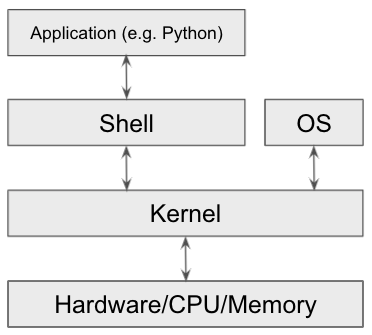
\includegraphics[width=6cm] {stack.png}
\end{figure}

Today's lecture is dedicated to giving you an overview of how a computer works. We will cover a lot to terms and concepts that often pop up when dealing with programming. This will also give you context on where Python is in the mess of things.

It is not necessary for you to understand the technical intricacies of everything that we'll cover. Don't worry if everything doesn't sink in.

\section{Hardware}

\textbf{1: Transistor} a semiconductor device that acts as a switch.

\begin{figure}[H]
	\centering
	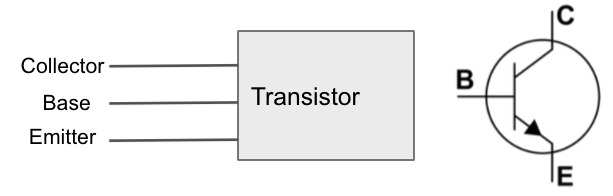
\includegraphics[width=9cm] {tran.png}
\end{figure}
Base HIGH: current passes from collector to emitter

Base LOW: current can not pass for collector to emitter

\textbf{2: Logic gate} collections of transistors that can compute basic logical operations. 

\begin{figure}[H]
	\centering
	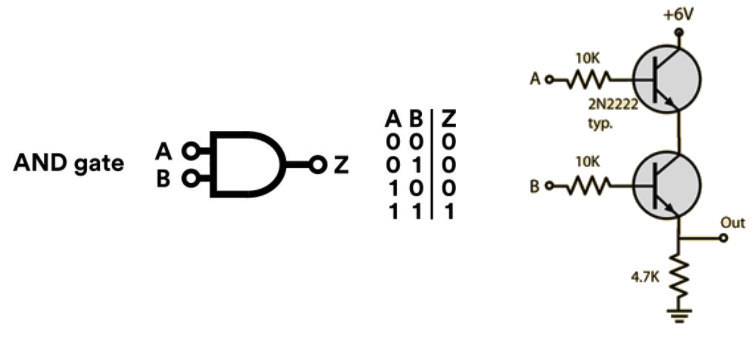
\includegraphics[width=11cm] {and.png}
\end{figure}

\textbf{3: CPU (central processing unit)} a collection of logic gate that can perform more complex operations: arithmetic, logic, controlling, input/output (i.e. reading from memory)

\begin{figure}[H]
	\centering
	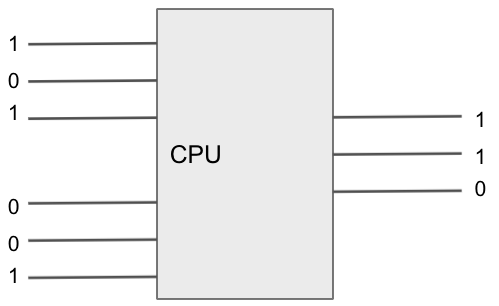
\includegraphics[width=8cm] {add.png}
	\caption{Simple diagram of adding $1+5=6$}
\end{figure}

\textbf{Machine code: }a low level programming language, written in binary, that a computer can directly execute. 

\textbf{Q: Are we done?}

No. While we have a computer, but how do we program it to do what we want?

\textbf{Past: }physical punch cards completed circuits to program inputs. PAINFUL!

\begin{figure}[H]
	\centering
	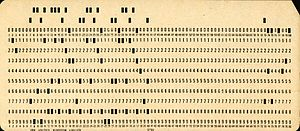
\includegraphics[width=6cm] {punch}
\end{figure}

\textbf{Now: }we have keyboards, monitors, and operating systems. But there's a bit more to the story...

\section{Kernel}
\begin{itemize}
    \item The core program that interfaces between the hardware and software (i.e. applications and programs we want to write).
    \item On startup, the kernel is the first program to start (...ignoring BIOS/UEFI and bootloader and I'm not a computer engineer...)
    \item The kernel is always running and has complete control over the computer.
    \item Kernel is the core of the operating system
\end{itemize}

\section{Operating System}
\begin{itemize}
    \item The OS is composed of a kernel and additional software to allow us to more easily interact with the computer. E.g. graphical user interface (GUI).
    \item Common OSs as Windows, Mac, and Linux. Each have a different kernel. A kernal/OS is not restricted to a single hardware platform. A PC can run both Windows and Linux.
    \item Not practical for remote access. 
\end{itemize}

\section{Shell}
\begin{itemize}
    \item A program that allows the user to directly interact with the kernel
    \item The shell program has a text-based interface often called the terminal or command line
    \item Greater control over OS
    \item Shell scripting (automate/program shell commands)
\end{itemize}

On Windows the default shell is DOS (Command Prompt application). On Mac and Linux machines, Bash is the default shell (Terminal application).

\textbf{Students should download Bash (Git Bash on Windows) before lecture.
}

\textbf{Demo}: bash commands (mention ``directory"$=$``folder")
\begin{itemize}
    \item pwd
    \item ls
    \item cd
    \item moving files to a folder based on file type
\end{itemize}

\section{Python}

Python is a high-level programming language with human-readable syntax.
\begin{itemize}
    \item Popular in research (many libraries)
    \item Fast code development (e.g. dynamic typing) 
\end{itemize}

\textbf{What happens when you run a Python program? (Interpreter)}
\begin{itemize}
    \item The interpreter \textit{interprets} and executes the python code
    \item You can think of the interpreter as translating your Python code into machine code for the computer to run.
    \item When you download Python, you're downloading the interpreter.
\end{itemize}

\begin{figure}[H]
	\centering
	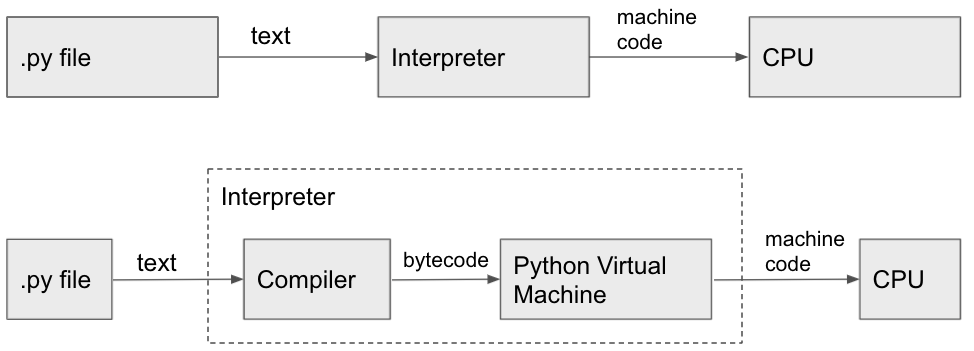
\includegraphics[width=13cm] {py}
\end{figure}

\textbf{Text Editors and IDEs}:
\begin{itemize}
    \item \textbf{Demo}: writing a Python program in a basic text editor and running on terminal.
    \item While you can write Python code on any text edit (try using Word and keeping your sanity at the same time...) there are special programs called integrated development environments that act as fancy text editors to write, run, test, and debug code.
    \item Example of IDE: PyCharm, Atom, Jupyter Notebook etc. \textbf{We will be using Jupyter Notebook: a very popular IDE in the lab!}
\end{itemize}

\section{Next Week}
\begin{itemize}
    \item Discussing how to use Jupyter Notebook
    \item Start learning about the Python language
\end{itemize}


\section{Homework}
\begin{itemize}
    \item Practice Bash commands
    \item Download Anaconda (for Python and Jupyter Notebook)
\end{itemize}



\end{document}
